\documentclass[1p]{elsarticle_modified}
%\bibliographystyle{elsarticle-num}

%\usepackage[colorlinks]{hyperref}
%\usepackage{abbrmath_seonhwa} %\Abb, \Ascr, \Acal ,\Abf, \Afrak
\usepackage{amsfonts}
\usepackage{amssymb}
\usepackage{amsmath}
\usepackage{amsthm}
\usepackage{scalefnt}
\usepackage{amsbsy}
\usepackage{kotex}
\usepackage{caption}
\usepackage{subfig}
\usepackage{color}
\usepackage{graphicx}
\usepackage{xcolor} %% white, black, red, green, blue, cyan, magenta, yellow
\usepackage{float}
\usepackage{setspace}
\usepackage{hyperref}

\usepackage{tikz}
\usetikzlibrary{arrows}

\usepackage{multirow}
\usepackage{array} % fixed length table
\usepackage{hhline}

%%%%%%%%%%%%%%%%%%%%%
\makeatletter
\renewcommand*\env@matrix[1][\arraystretch]{%
	\edef\arraystretch{#1}%
	\hskip -\arraycolsep
	\let\@ifnextchar\new@ifnextchar
	\array{*\c@MaxMatrixCols c}}
\makeatother %https://tex.stackexchange.com/questions/14071/how-can-i-increase-the-line-spacing-in-a-matrix
%%%%%%%%%%%%%%%

\usepackage[normalem]{ulem}

\newcommand{\msout}[1]{\ifmmode\text{\sout{\ensuremath{#1}}}\else\sout{#1}\fi}
%SOURCE: \msout is \stkout macro in https://tex.stackexchange.com/questions/20609/strikeout-in-math-mode

\newcommand{\cancel}[1]{
	\ifmmode
	{\color{red}\msout{#1}}
	\else
	{\color{red}\sout{#1}}
	\fi
}

\newcommand{\add}[1]{
	{\color{blue}\uwave{#1}}
}

\newcommand{\replace}[2]{
	\ifmmode
	{\color{red}\msout{#1}}{\color{blue}\uwave{#2}}
	\else
	{\color{red}\sout{#1}}{\color{blue}\uwave{#2}}
	\fi
}

\newcommand{\Sol}{\mathcal{S}} %segment
\newcommand{\D}{D} %diagram
\newcommand{\A}{\mathcal{A}} %arc


%%%%%%%%%%%%%%%%%%%%%%%%%%%%%5 test

\def\sl{\operatorname{\textup{SL}}(2,\Cbb)}
\def\psl{\operatorname{\textup{PSL}}(2,\Cbb)}
\def\quan{\mkern 1mu \triangleright \mkern 1mu}

\theoremstyle{definition}
\newtheorem{thm}{Theorem}[section]
\newtheorem{prop}[thm]{Proposition}
\newtheorem{lem}[thm]{Lemma}
\newtheorem{ques}[thm]{Question}
\newtheorem{cor}[thm]{Corollary}
\newtheorem{defn}[thm]{Definition}
\newtheorem{exam}[thm]{Example}
\newtheorem{rmk}[thm]{Remark}
\newtheorem{alg}[thm]{Algorithm}

\newcommand{\I}{\sqrt{-1}}
\begin{document}

%\begin{frontmatter}
%
%\title{Boundary parabolic representations of knots up to 8 crossings}
%
%%% Group authors per affiliation:
%\author{Yunhi Cho} 
%\address{Department of Mathematics, University of Seoul, Seoul, Korea}
%\ead{yhcho@uos.ac.kr}
%
%
%\author{Seonhwa Kim} %\fnref{s_kim}}
%\address{Center for Geometry and Physics, Institute for Basic Science, Pohang, 37673, Korea}
%\ead{ryeona17@ibs.re.kr}
%
%\author{Hyuk Kim}
%\address{Department of Mathematical Sciences, Seoul National University, Seoul 08826, Korea}
%\ead{hyukkim@snu.ac.kr}
%
%\author{Seokbeom Yoon}
%\address{Department of Mathematical Sciences, Seoul National University, Seoul, 08826,  Korea}
%\ead{sbyoon15@snu.ac.kr}
%
%\begin{abstract}
%We find all boundary parabolic representation of knots up to 8 crossings.
%
%\end{abstract}
%\begin{keyword}
%    \MSC[2010] 57M25 
%\end{keyword}
%
%\end{frontmatter}

%\linenumbers
%\tableofcontents
%
\newcommand\colored[1]{\textcolor{white}{\rule[-0.35ex]{0.8em}{1.4ex}}\kern-0.8em\color{red} #1}%
%\newcommand\colored[1]{\textcolor{white}{ #1}\kern-2.17ex	\textcolor{white}{ #1}\kern-1.81ex	\textcolor{white}{ #1}\kern-2.15ex\color{red}#1	}

{\Large $\underline{12n_{0510}~(K12n_{0510})}$}

\setlength{\tabcolsep}{10pt}
\renewcommand{\arraystretch}{1.6}
\vspace{1cm}\begin{tabular}{m{100pt}>{\centering\arraybackslash}m{274pt}}
\multirow{5}{120pt}{
	\centering
	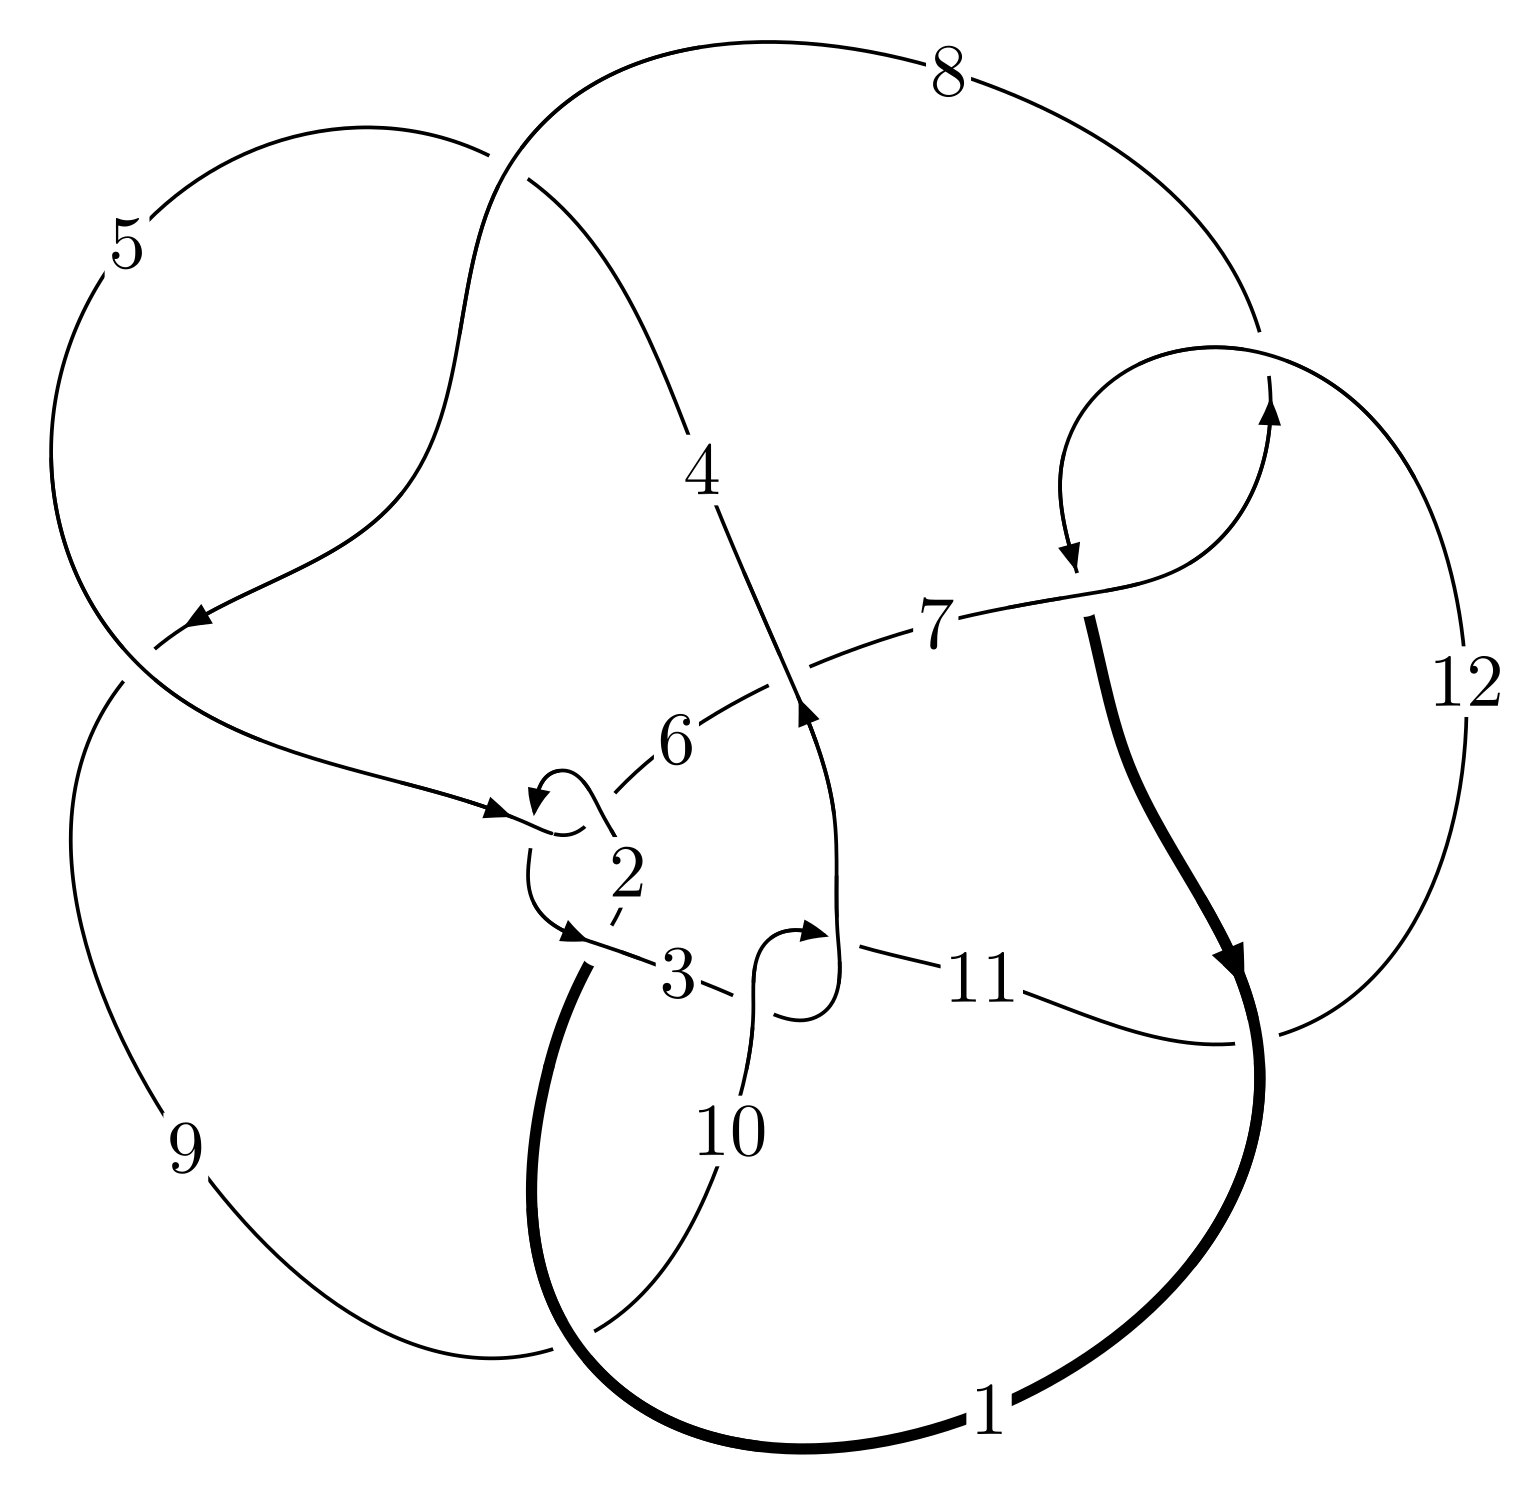
\includegraphics[width=112pt]{../../../GIT/diagram.site/Diagrams/png/2599_12n_0510.png}\\
\ \ \ A knot diagram\footnotemark}&
\allowdisplaybreaks
\textbf{Linearized knot diagam} \\
\cline{2-2}
 &
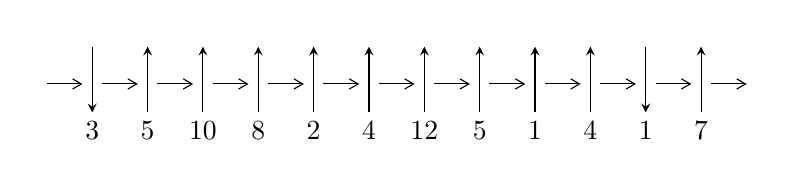
\begin{tikzpicture}[x=20pt, y=17pt]
	% nodes
	\node (C0) at (0, 0) {};
	\node (C1) at (1, 0) {};
	\node (C1U) at (1, +1) {};
	\node (C1D) at (1, -1) {3};

	\node (C2) at (2, 0) {};
	\node (C2U) at (2, +1) {};
	\node (C2D) at (2, -1) {5};

	\node (C3) at (3, 0) {};
	\node (C3U) at (3, +1) {};
	\node (C3D) at (3, -1) {10};

	\node (C4) at (4, 0) {};
	\node (C4U) at (4, +1) {};
	\node (C4D) at (4, -1) {8};

	\node (C5) at (5, 0) {};
	\node (C5U) at (5, +1) {};
	\node (C5D) at (5, -1) {2};

	\node (C6) at (6, 0) {};
	\node (C6U) at (6, +1) {};
	\node (C6D) at (6, -1) {4};

	\node (C7) at (7, 0) {};
	\node (C7U) at (7, +1) {};
	\node (C7D) at (7, -1) {12};

	\node (C8) at (8, 0) {};
	\node (C8U) at (8, +1) {};
	\node (C8D) at (8, -1) {5};

	\node (C9) at (9, 0) {};
	\node (C9U) at (9, +1) {};
	\node (C9D) at (9, -1) {1};

	\node (C10) at (10, 0) {};
	\node (C10U) at (10, +1) {};
	\node (C10D) at (10, -1) {4};

	\node (C11) at (11, 0) {};
	\node (C11U) at (11, +1) {};
	\node (C11D) at (11, -1) {1};

	\node (C12) at (12, 0) {};
	\node (C12U) at (12, +1) {};
	\node (C12D) at (12, -1) {7};
	\node (C13) at (13, 0) {};

	% arrows
	\draw[->,>={angle 60}]
	(C0) edge (C1) (C1) edge (C2) (C2) edge (C3) (C3) edge (C4) (C4) edge (C5) (C5) edge (C6) (C6) edge (C7) (C7) edge (C8) (C8) edge (C9) (C9) edge (C10) (C10) edge (C11) (C11) edge (C12) (C12) edge (C13) ;	\draw[->,>=stealth]
	(C1U) edge (C1D) (C2D) edge (C2U) (C3D) edge (C3U) (C4D) edge (C4U) (C5D) edge (C5U) (C6D) edge (C6U) (C7D) edge (C7U) (C8D) edge (C8U) (C9D) edge (C9U) (C10D) edge (C10U) (C11U) edge (C11D) (C12D) edge (C12U) ;
	\end{tikzpicture} \\
\hhline{~~} \\& 
\textbf{Solving Sequence} \\ \cline{2-2} 
 &
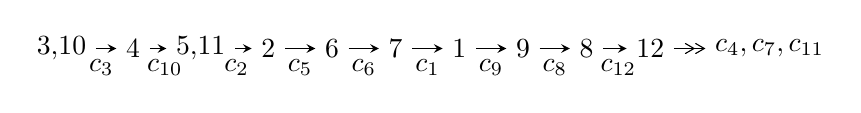
\begin{tikzpicture}[x=23pt, y=7pt]
	% node
	\node (A0) at (-1/8, 0) {3,10};
	\node (A1) at (1, 0) {4};
	\node (A2) at (33/16, 0) {5,11};
	\node (A3) at (25/8, 0) {2};
	\node (A4) at (33/8, 0) {6};
	\node (A5) at (41/8, 0) {7};
	\node (A6) at (49/8, 0) {1};
	\node (A7) at (57/8, 0) {9};
	\node (A8) at (65/8, 0) {8};
	\node (A9) at (73/8, 0) {12};
	\node (C1) at (1/2, -1) {$c_{3}$};
	\node (C2) at (3/2, -1) {$c_{10}$};
	\node (C3) at (21/8, -1) {$c_{2}$};
	\node (C4) at (29/8, -1) {$c_{5}$};
	\node (C5) at (37/8, -1) {$c_{6}$};
	\node (C6) at (45/8, -1) {$c_{1}$};
	\node (C7) at (53/8, -1) {$c_{9}$};
	\node (C8) at (61/8, -1) {$c_{8}$};
	\node (C9) at (69/8, -1) {$c_{12}$};
	\node (A10) at (11, 0) {$c_{4},c_{7},c_{11}$};

	% edge
	\draw[->,>=stealth]	
	(A0) edge (A1) (A1) edge (A2) (A2) edge (A3) (A3) edge (A4) (A4) edge (A5) (A5) edge (A6) (A6) edge (A7) (A7) edge (A8) (A8) edge (A9) ;
	\draw[->>,>={angle 60}]	
	(A9) edge (A10);
\end{tikzpicture} \\ 

\end{tabular} \\

\footnotetext{
The image of knot diagram is generated by the software ``\textbf{Draw programme}" developed by Andrew Bartholomew(\url{http://www.layer8.co.uk/maths/draw/index.htm\#Running-draw}), where we modified some parts for our purpose(\url{https://github.com/CATsTAILs/LinksPainter}).
}\phantom \\ \newline 
\centering \textbf{Ideals for irreducible components\footnotemark of $X_{\text{par}}$} 
 
\begin{align*}
I^u_{1}&=\langle 
u^8-4 u^7+8 u^6-8 u^5+4 u^4+u^2+b-2 u+1,\;- u^8+4 u^7-8 u^6+8 u^5-4 u^4- u^3+a+2 u-2,\\
\phantom{I^u_{1}}&\phantom{= \langle  }u^9-5 u^8+12 u^7-16 u^6+12 u^5-3 u^4- u^3- u^2+3 u-1\rangle \\
I^u_{2}&=\langle 
u^2 a+u^2+b,\;- u^9 a+4 u^9+\cdots+2 a-1,\;u^{10}+2 u^9+u^8- u^7+2 u^6+5 u^5+2 u^4-4 u^3-3 u^2+u+1\rangle \\
I^u_{3}&=\langle 
-9 u^9+29 u^8-20 u^7-81 u^6+207 u^5-123 u^4-256 u^3+576 u^2+16 b-472 u+176,\\
\phantom{I^u_{3}}&\phantom{= \langle  }13 u^9-43 u^8+34 u^7+113 u^6-309 u^5+217 u^4+350 u^3-876 u^2+32 a+776 u-320,\\
\phantom{I^u_{3}}&\phantom{= \langle  }u^{10}-5 u^9+8 u^8+5 u^7-39 u^6+55 u^5+4 u^4-116 u^3+168 u^2-112 u+32\rangle \\
I^u_{4}&=\langle 
u^8-2 u^7-2 u^6+6 u^5-2 u^4-4 u^3+5 u^2+b-1,\;- u^8+2 u^7+2 u^6-6 u^5+2 u^4+3 u^3-4 u^2+a+2 u,\\
\phantom{I^u_{4}}&\phantom{= \langle  }u^9- u^8-4 u^7+4 u^6+4 u^5-5 u^4+u^3+3 u^2- u-1\rangle \\
I^u_{5}&=\langle 
4 u^{19}-5 u^{18}+\cdots+8 b-34,\;-8 u^{19} a-62 u^{19}+\cdots-86 a-198,\;u^{20}+2 u^{19}+\cdots+2 u-1\rangle \\
I^u_{6}&=\langle 
u^2 a+u^2+b,\;u^2 a+a^2+u^2+a+u-1,\;u^3- u-1\rangle \\
I^u_{7}&=\langle 
- a u+b+a- u+1,\;a^2-2 a u- a+u+3,\;u^2+u-1\rangle \\
\\
\end{align*}
\raggedright * 7 irreducible components of $\dim_{\mathbb{C}}=0$, with total 98 representations.\\
\footnotetext{All coefficients of polynomials are rational numbers. But the coefficients are sometimes approximated in decimal forms when there is not enough margin.}
\newpage
\renewcommand{\arraystretch}{1}
\centering \section*{I. $I^u_{1}= \langle u^8-4 u^7+8 u^6-8 u^5+4 u^4+u^2+b-2 u+1,\;- u^8+4 u^7+\cdots+a-2,\;u^9-5 u^8+\cdots+3 u-1 \rangle$}
\flushleft \textbf{(i) Arc colorings}\\
\begin{tabular}{m{7pt} m{180pt} m{7pt} m{180pt} }
\flushright $a_{3}=$&$\begin{pmatrix}1\\0\end{pmatrix}$ \\
\flushright $a_{10}=$&$\begin{pmatrix}0\\u\end{pmatrix}$ \\
\flushright $a_{4}=$&$\begin{pmatrix}1\\- u^2\end{pmatrix}$ \\
\flushright $a_{5}=$&$\begin{pmatrix}u^8-4 u^7+8 u^6-8 u^5+4 u^4+u^3-2 u+2\\- u^8+4 u^7-8 u^6+8 u^5-4 u^4- u^2+2 u-1\end{pmatrix}$ \\
\flushright $a_{11}=$&$\begin{pmatrix}u\\- u^3+u\end{pmatrix}$ \\
\flushright $a_{2}=$&$\begin{pmatrix}u^7-3 u^6+5 u^5-4 u^4+2 u^3+u\\- u^8+3 u^7-4 u^6+u^5+2 u^4-2 u^3- u^2+u\end{pmatrix}$ \\
\flushright $a_{6}=$&$\begin{pmatrix}u^8-3 u^7+5 u^6-4 u^5+2 u^4+u^3+1\\-2 u^8+7 u^7-12 u^6+10 u^5-4 u^4- u^3- u^2+2 u-1\end{pmatrix}$ \\
\flushright $a_{7}=$&$\begin{pmatrix}2 u^8-8 u^7+15 u^6-14 u^5+5 u^4+3 u^3- u^2-3 u+2\\u^7-3 u^6+5 u^5-4 u^4+u^3+u^2+u-1\end{pmatrix}$ \\
\flushright $a_{1}=$&$\begin{pmatrix}- u^8+4 u^7-7 u^6+6 u^5-2 u^4- u^2+2 u\\- u^8+3 u^7-4 u^6+u^5+2 u^4-2 u^3- u^2+u\end{pmatrix}$ \\
\flushright $a_{9}=$&$\begin{pmatrix}- u^2\\u^4- u^3+u\end{pmatrix}$ \\
\flushright $a_{8}=$&$\begin{pmatrix}- u^8+4 u^7-8 u^6+8 u^5-4 u^4- u^3+u-1\\u^8-4 u^7+8 u^6-8 u^5+4 u^4+u^3- u^2- u+1\end{pmatrix}$ \\
\flushright $a_{12}=$&$\begin{pmatrix}u^3- u^2+u\\- u^5+2 u^4-2 u^3+u\end{pmatrix}$\\&\end{tabular}
\flushleft \textbf{(ii) Obstruction class $= -1$}\\~\\
\flushleft \textbf{(iii) Cusp Shapes $= -4 u^7+18 u^6-32 u^5+24 u^4-12 u^2+2 u+15$}\\~\\
\newpage\renewcommand{\arraystretch}{1}
\flushleft \textbf{(iv) u-Polynomials at the component}\newline \\
\begin{tabular}{m{50pt}|m{274pt}}
Crossings & \hspace{64pt}u-Polynomials at each crossing \\
\hline $$\begin{aligned}c_{1},c_{11}\end{aligned}$$&$\begin{aligned}
&u^9+5 u^8+11 u^7+10 u^6- u^5-5 u^4+9 u^3+14 u^2+4 u-1
\end{aligned}$\\
\hline $$\begin{aligned}c_{2},c_{5},c_{7}\\c_{12}\end{aligned}$$&$\begin{aligned}
&u^9+3 u^8+7 u^7+10 u^6+11 u^5+9 u^4+5 u^3+2 u^2-1
\end{aligned}$\\
\hline $$\begin{aligned}c_{3},c_{4},c_{8}\\c_{10}\end{aligned}$$&$\begin{aligned}
&u^9-5 u^8+12 u^7-16 u^6+12 u^5-3 u^4- u^3- u^2+3 u-1
\end{aligned}$\\
\hline $$\begin{aligned}c_{6},c_{9}\end{aligned}$$&$\begin{aligned}
&u^9+u^8+4 u^7+u^6+11 u^5+u^4+11 u^3+7 u^2+u-1
\end{aligned}$\\
\hline
\end{tabular}\\~\\
\newpage\renewcommand{\arraystretch}{1}
\flushleft \textbf{(v) Riley Polynomials at the component}\newline \\
\begin{tabular}{m{50pt}|m{274pt}}
Crossings & \hspace{64pt}Riley Polynomials at each crossing \\
\hline $$\begin{aligned}c_{1},c_{11}\end{aligned}$$&$\begin{aligned}
&y^9-3 y^8+19 y^7-54 y^6+167 y^5-225 y^4+233 y^3-134 y^2+44 y-1
\end{aligned}$\\
\hline $$\begin{aligned}c_{2},c_{5},c_{7}\\c_{12}\end{aligned}$$&$\begin{aligned}
&y^9+5 y^8+11 y^7+10 y^6- y^5-5 y^4+9 y^3+14 y^2+4 y-1
\end{aligned}$\\
\hline $$\begin{aligned}c_{3},c_{4},c_{8}\\c_{10}\end{aligned}$$&$\begin{aligned}
&y^9- y^8+8 y^7+20 y^5-3 y^4+35 y^3-13 y^2+7 y-1
\end{aligned}$\\
\hline $$\begin{aligned}c_{6},c_{9}\end{aligned}$$&$\begin{aligned}
&y^9+7 y^8+36 y^7+107 y^6+195 y^5+237 y^4+131 y^3-25 y^2+15 y-1
\end{aligned}$\\
\hline
\end{tabular}\\~\\
\newpage\flushleft \textbf{(vi) Complex Volumes and Cusp Shapes}
$$\begin{array}{c|c|c}  
\text{Solutions to }I^u_{1}& \I (\text{vol} + \sqrt{-1}CS) & \text{Cusp shape}\\
 \hline 
\begin{aligned}
u &= \phantom{-}1.000250 + 0.725181 I \\
a &= -1.000710 + 0.653784 I \\
b &= \phantom{-}0.948795 - 0.309253 I\end{aligned}
 & \phantom{-}0.91788 + 5.42837 I & \phantom{-}11.84517 - 4.00961 I \\ \hline\begin{aligned}
u &= \phantom{-}1.000250 - 0.725181 I \\
a &= -1.000710 - 0.653784 I \\
b &= \phantom{-}0.948795 + 0.309253 I\end{aligned}
 & \phantom{-}0.91788 - 5.42837 I & \phantom{-}11.84517 + 4.00961 I \\ \hline\begin{aligned}
u &= \phantom{-}0.546415 + 1.108600 I \\
a &= -0.230267 - 0.335909 I \\
b &= \phantom{-}0.309218 - 1.245070 I\end{aligned}
 & -9.16918 - 1.97699 I & \phantom{-}1.47834 + 1.39149 I \\ \hline\begin{aligned}
u &= \phantom{-}0.546415 - 1.108600 I \\
a &= -0.230267 + 0.335909 I \\
b &= \phantom{-}0.309218 + 1.245070 I\end{aligned}
 & -9.16918 + 1.97699 I & \phantom{-}1.47834 - 1.39149 I \\ \hline\begin{aligned}
u &= -0.519685 + 0.388914 I \\
a &= \phantom{-}1.137270 - 0.230863 I \\
b &= -0.160625 + 0.891368 I\end{aligned}
 & -2.04430 - 1.72035 I & \phantom{-}4.21443 + 4.65394 I \\ \hline\begin{aligned}
u &= -0.519685 - 0.388914 I \\
a &= \phantom{-}1.137270 + 0.230863 I \\
b &= -0.160625 - 0.891368 I\end{aligned}
 & -2.04430 + 1.72035 I & \phantom{-}4.21443 - 4.65394 I \\ \hline\begin{aligned}
u &= \phantom{-}1.26544 + 0.92224 I \\
a &= -1.55365 + 0.07913 I \\
b &= \phantom{-}0.600380 + 1.232850 I\end{aligned}
 & -4.8606 + 16.8243 I & \phantom{-}6.88008 - 9.57741 I \\ \hline\begin{aligned}
u &= \phantom{-}1.26544 - 0.92224 I \\
a &= -1.55365 - 0.07913 I \\
b &= \phantom{-}0.600380 - 1.232850 I\end{aligned}
 & -4.8606 - 16.8243 I & \phantom{-}6.88008 + 9.57741 I \\ \hline\begin{aligned}
u &= \phantom{-}0.415171\phantom{ +0.000000I} \\
a &= \phantom{-}1.29473\phantom{ +0.000000I} \\
b &= -0.395535\phantom{ +0.000000I}\end{aligned}
 & \phantom{-}0.703597\phantom{ +0.000000I} & \phantom{-}14.1640\phantom{ +0.000000I}\\
 \hline 
 \end{array}$$\newpage\newpage\renewcommand{\arraystretch}{1}
\centering \section*{II. $I^u_{2}= \langle u^2 a+u^2+b,\;- u^9 a+4 u^9+\cdots+2 a-1,\;u^{10}+2 u^9+\cdots+u+1 \rangle$}
\flushleft \textbf{(i) Arc colorings}\\
\begin{tabular}{m{7pt} m{180pt} m{7pt} m{180pt} }
\flushright $a_{3}=$&$\begin{pmatrix}1\\0\end{pmatrix}$ \\
\flushright $a_{10}=$&$\begin{pmatrix}0\\u\end{pmatrix}$ \\
\flushright $a_{4}=$&$\begin{pmatrix}1\\- u^2\end{pmatrix}$ \\
\flushright $a_{5}=$&$\begin{pmatrix}a\\- u^2 a- u^2\end{pmatrix}$ \\
\flushright $a_{11}=$&$\begin{pmatrix}u\\- u^3+u\end{pmatrix}$ \\
\flushright $a_{2}=$&$\begin{pmatrix}- u^9 a+3 u^9+\cdots-2 u+3\\u^8 a-2 u^9+\cdots+u-2\end{pmatrix}$ \\
\flushright $a_{6}=$&$\begin{pmatrix}-2 u^9 a-3 u^8 a+\cdots-2 a-2\\u^9 a+u^9+\cdots+2 a+3\end{pmatrix}$ \\
\flushright $a_{7}=$&$\begin{pmatrix}- u^9 a+2 u^9+\cdots- a-2 u\\u^9 a+u^8 a+\cdots+a+1\end{pmatrix}$ \\
\flushright $a_{1}=$&$\begin{pmatrix}- u^9 a+u^9+\cdots- u+1\\u^8 a-2 u^9+\cdots+u-2\end{pmatrix}$ \\
\flushright $a_{9}=$&$\begin{pmatrix}u^9 a- u^9+\cdots+a-1\\- u^3 a- u^3+a u\end{pmatrix}$ \\
\flushright $a_{8}=$&$\begin{pmatrix}u^9 a- u^9+\cdots+a-1\\a u\end{pmatrix}$ \\
\flushright $a_{12}=$&$\begin{pmatrix}u^9 a- u^9+\cdots+a-1\\u^8+u^7- u^5+3 u^4+2 u^3-3 u\end{pmatrix}$\\&\end{tabular}
\flushleft \textbf{(ii) Obstruction class $= -1$}\\~\\
\flushleft \textbf{(iii) Cusp Shapes $= 11 u^9+12 u^8-8 u^7-19 u^6+32 u^5+32 u^4-25 u^3-59 u^2+4 u+39$}\\~\\
\newpage\renewcommand{\arraystretch}{1}
\flushleft \textbf{(iv) u-Polynomials at the component}\newline \\
\begin{tabular}{m{50pt}|m{274pt}}
Crossings & \hspace{64pt}u-Polynomials at each crossing \\
\hline $$\begin{aligned}c_{1},c_{11}\end{aligned}$$&$\begin{aligned}
&u^{20}+8 u^{19}+\cdots-512 u+1024
\end{aligned}$\\
\hline $$\begin{aligned}c_{2},c_{5},c_{7}\\c_{12}\end{aligned}$$&$\begin{aligned}
&u^{20}+6 u^{19}+\cdots+192 u+32
\end{aligned}$\\
\hline $$\begin{aligned}c_{3},c_{4},c_{8}\\c_{10}\end{aligned}$$&$\begin{aligned}
&(u^{10}+2 u^9+u^8- u^7+2 u^6+5 u^5+2 u^4-4 u^3-3 u^2+u+1)^2
\end{aligned}$\\
\hline $$\begin{aligned}c_{6},c_{9}\end{aligned}$$&$\begin{aligned}
&u^{20}+2 u^{19}+\cdots-13 u^2+1
\end{aligned}$\\
\hline
\end{tabular}\\~\\
\newpage\renewcommand{\arraystretch}{1}
\flushleft \textbf{(v) Riley Polynomials at the component}\newline \\
\begin{tabular}{m{50pt}|m{274pt}}
Crossings & \hspace{64pt}Riley Polynomials at each crossing \\
\hline $$\begin{aligned}c_{1},c_{11}\end{aligned}$$&$\begin{aligned}
&y^{20}+8 y^{19}+\cdots+655360 y+1048576
\end{aligned}$\\
\hline $$\begin{aligned}c_{2},c_{5},c_{7}\\c_{12}\end{aligned}$$&$\begin{aligned}
&y^{20}+8 y^{19}+\cdots-512 y+1024
\end{aligned}$\\
\hline $$\begin{aligned}c_{3},c_{4},c_{8}\\c_{10}\end{aligned}$$&$\begin{aligned}
&(y^{10}-2 y^9+9 y^8-13 y^7+28 y^6-33 y^5+36 y^4-34 y^3+21 y^2-7 y+1)^{2}
\end{aligned}$\\
\hline $$\begin{aligned}c_{6},c_{9}\end{aligned}$$&$\begin{aligned}
&y^{20}+24 y^{19}+\cdots-26 y+1
\end{aligned}$\\
\hline
\end{tabular}\\~\\
\newpage\flushleft \textbf{(vi) Complex Volumes and Cusp Shapes}
$$\begin{array}{c|c|c}  
\text{Solutions to }I^u_{2}& \I (\text{vol} + \sqrt{-1}CS) & \text{Cusp shape}\\
 \hline 
\begin{aligned}
u &= -0.697487 + 0.893220 I \\
a &= -0.662772 - 0.575220 I \\
b &= \phantom{-}0.821731 + 0.241096 I\end{aligned}
 & -4.56796 - 1.72827 I & \phantom{-}5.99377 + 2.10096 I \\ \hline\begin{aligned}
u &= -0.697487 + 0.893220 I \\
a &= \phantom{-}0.0120261 + 0.0747158 I \\
b &= \phantom{-}0.222000 + 1.284270 I\end{aligned}
 & -4.56796 - 1.72827 I & \phantom{-}5.99377 + 2.10096 I \\ \hline\begin{aligned}
u &= -0.697487 - 0.893220 I \\
a &= -0.662772 + 0.575220 I \\
b &= \phantom{-}0.821731 - 0.241096 I\end{aligned}
 & -4.56796 + 1.72827 I & \phantom{-}5.99377 - 2.10096 I \\ \hline\begin{aligned}
u &= -0.697487 - 0.893220 I \\
a &= \phantom{-}0.0120261 - 0.0747158 I \\
b &= \phantom{-}0.222000 - 1.284270 I\end{aligned}
 & -4.56796 + 1.72827 I & \phantom{-}5.99377 - 2.10096 I \\ \hline\begin{aligned}
u &= -0.693459 + 0.193871 I \\
a &= \phantom{-}1.50091 - 0.64277 I \\
b &= -0.935824 + 0.957395 I\end{aligned}
 & \phantom{-}2.81596 - 6.19567 I & \phantom{-}19.0021 + 9.7994 I \\ \hline\begin{aligned}
u &= -0.693459 + 0.193871 I \\
a &= -3.12443 + 0.88317 I \\
b &= \phantom{-}0.704293 - 0.962732 I\end{aligned}
 & \phantom{-}2.81596 - 6.19567 I & \phantom{-}19.0021 + 9.7994 I \\ \hline\begin{aligned}
u &= -0.693459 - 0.193871 I \\
a &= \phantom{-}1.50091 + 0.64277 I \\
b &= -0.935824 - 0.957395 I\end{aligned}
 & \phantom{-}2.81596 + 6.19567 I & \phantom{-}19.0021 - 9.7994 I \\ \hline\begin{aligned}
u &= -0.693459 - 0.193871 I \\
a &= -3.12443 - 0.88317 I \\
b &= \phantom{-}0.704293 + 0.962732 I\end{aligned}
 & \phantom{-}2.81596 + 6.19567 I & \phantom{-}19.0021 - 9.7994 I \\ \hline\begin{aligned}
u &= \phantom{-}0.862296 + 0.948082 I \\
a &= -1.67900 + 0.41333 I \\
b &= \phantom{-}0.570373 + 1.174400 I\end{aligned}
 & -7.29651 + 6.88238 I & \phantom{-}4.01797 - 5.83705 I \\ \hline\begin{aligned}
u &= \phantom{-}0.862296 + 0.948082 I \\
a &= -0.166644 + 0.078095 I \\
b &= \phantom{-}0.257113 - 1.350450 I\end{aligned}
 & -7.29651 + 6.88238 I & \phantom{-}4.01797 - 5.83705 I\\
 \hline 
 \end{array}$$\newpage$$\begin{array}{c|c|c}  
\text{Solutions to }I^u_{2}& \I (\text{vol} + \sqrt{-1}CS) & \text{Cusp shape}\\
 \hline 
\begin{aligned}
u &= \phantom{-}0.862296 - 0.948082 I \\
a &= -1.67900 - 0.41333 I \\
b &= \phantom{-}0.570373 - 1.174400 I\end{aligned}
 & -7.29651 - 6.88238 I & \phantom{-}4.01797 + 5.83705 I \\ \hline\begin{aligned}
u &= \phantom{-}0.862296 - 0.948082 I \\
a &= -0.166644 - 0.078095 I \\
b &= \phantom{-}0.257113 + 1.350450 I\end{aligned}
 & -7.29651 - 6.88238 I & \phantom{-}4.01797 + 5.83705 I \\ \hline\begin{aligned}
u &= \phantom{-}0.663837 + 0.151994 I \\
a &= \phantom{-}1.58914 + 0.48669 I \\
b &= -0.982955 - 0.725714 I\end{aligned}
 & \phantom{-}3.48993 + 0.66365 I & \phantom{-}16.4607 - 8.1518 I \\ \hline\begin{aligned}
u &= \phantom{-}0.663837 + 0.151994 I \\
a &= -1.75895 + 2.14112 I \\
b &= \phantom{-}0.748997 - 0.740931 I\end{aligned}
 & \phantom{-}3.48993 + 0.66365 I & \phantom{-}16.4607 - 8.1518 I \\ \hline\begin{aligned}
u &= \phantom{-}0.663837 - 0.151994 I \\
a &= \phantom{-}1.58914 - 0.48669 I \\
b &= -0.982955 + 0.725714 I\end{aligned}
 & \phantom{-}3.48993 - 0.66365 I & \phantom{-}16.4607 + 8.1518 I \\ \hline\begin{aligned}
u &= \phantom{-}0.663837 - 0.151994 I \\
a &= -1.75895 - 2.14112 I \\
b &= \phantom{-}0.748997 + 0.740931 I\end{aligned}
 & \phantom{-}3.48993 - 0.66365 I & \phantom{-}16.4607 + 8.1518 I \\ \hline\begin{aligned}
u &= -1.135190 + 0.826360 I \\
a &= -1.031390 - 0.513255 I \\
b &= \phantom{-}0.981958 + 0.252022 I\end{aligned}
 & -1.84362 - 11.11570 I & \phantom{-}9.52549 + 6.91894 I \\ \hline\begin{aligned}
u &= -1.135190 + 0.826360 I \\
a &= -1.67888 - 0.10717 I \\
b &= \phantom{-}0.612314 - 1.208760 I\end{aligned}
 & -1.84362 - 11.11570 I & \phantom{-}9.52549 + 6.91894 I \\ \hline\begin{aligned}
u &= -1.135190 - 0.826360 I \\
a &= -1.031390 + 0.513255 I \\
b &= \phantom{-}0.981958 - 0.252022 I\end{aligned}
 & -1.84362 + 11.11570 I & \phantom{-}9.52549 - 6.91894 I \\ \hline\begin{aligned}
u &= -1.135190 - 0.826360 I \\
a &= -1.67888 + 0.10717 I \\
b &= \phantom{-}0.612314 + 1.208760 I\end{aligned}
 & -1.84362 + 11.11570 I & \phantom{-}9.52549 - 6.91894 I\\
 \hline 
 \end{array}$$\newpage\newpage\renewcommand{\arraystretch}{1}
\centering \section*{III. $I^u_{3}= \langle -9 u^9+29 u^8+\cdots+16 b+176,\;13 u^9-43 u^8+\cdots+32 a-320,\;u^{10}-5 u^9+\cdots-112 u+32 \rangle$}
\flushleft \textbf{(i) Arc colorings}\\
\begin{tabular}{m{7pt} m{180pt} m{7pt} m{180pt} }
\flushright $a_{3}=$&$\begin{pmatrix}1\\0\end{pmatrix}$ \\
\flushright $a_{10}=$&$\begin{pmatrix}0\\u\end{pmatrix}$ \\
\flushright $a_{4}=$&$\begin{pmatrix}1\\- u^2\end{pmatrix}$ \\
\flushright $a_{5}=$&$\begin{pmatrix}-\frac{13}{32} u^9+\frac{43}{32} u^8+\cdots-\frac{97}{4} u+10\\\frac{9}{16} u^9-\frac{29}{16} u^8+\cdots+\frac{59}{2} u-11\end{pmatrix}$ \\
\flushright $a_{11}=$&$\begin{pmatrix}u\\- u^3+u\end{pmatrix}$ \\
\flushright $a_{2}=$&$\begin{pmatrix}-\frac{37}{16} u^9+\frac{133}{16} u^8+\cdots-\frac{571}{4} u+50\\u^9-\frac{31}{8} u^8+\cdots+73 u-26\end{pmatrix}$ \\
\flushright $a_{6}=$&$\begin{pmatrix}-\frac{3}{16} u^9+\frac{7}{16} u^8+\cdots-8 u+\frac{9}{2}\\\frac{1}{2} u^9-\frac{11}{8} u^8+\cdots+\frac{33}{2} u-6\end{pmatrix}$ \\
\flushright $a_{7}=$&$\begin{pmatrix}-0.812500 u^{9}+2.68750 u^{8}+\cdots-41.5000 u+14.5000\\\frac{3}{2} u^9-\frac{43}{8} u^8+\cdots+\frac{189}{2} u-34\end{pmatrix}$ \\
\flushright $a_{1}=$&$\begin{pmatrix}-\frac{21}{16} u^9+\frac{71}{16} u^8+\cdots-\frac{279}{4} u+24\\u^9-\frac{31}{8} u^8+\cdots+73 u-26\end{pmatrix}$ \\
\flushright $a_{9}=$&$\begin{pmatrix}1.81250 u^{9}-6.06250 u^{8}+\cdots+100.250 u-34.5000\\-\frac{15}{8} u^9+\frac{13}{2} u^8+\cdots-\frac{217}{2} u+38\end{pmatrix}$ \\
\flushright $a_{8}=$&$\begin{pmatrix}-\frac{1}{16} u^8+\frac{3}{16} u^7+\cdots+\frac{7}{2} u-\frac{5}{2}\\\frac{1}{16} u^9-\frac{3}{16} u^8+\cdots-\frac{9}{2} u^2+\frac{7}{2} u\end{pmatrix}$ \\
\flushright $a_{12}=$&$\begin{pmatrix}-1.18750 u^{9}+4.06250 u^{8}+\cdots-67.2500 u+23.5000\\u^9-\frac{29}{8} u^8+\cdots+\frac{127}{2} u-22\end{pmatrix}$\\&\end{tabular}
\flushleft \textbf{(ii) Obstruction class $= -1$}\\~\\
\flushleft \textbf{(iii) Cusp Shapes $= -12 u^9+42 u^8-32 u^7-110 u^6+302 u^5-200 u^4-356 u^3+854 u^2-716 u+262$}\\~\\
\newpage\renewcommand{\arraystretch}{1}
\flushleft \textbf{(iv) u-Polynomials at the component}\newline \\
\begin{tabular}{m{50pt}|m{274pt}}
Crossings & \hspace{64pt}u-Polynomials at each crossing \\
\hline $$\begin{aligned}c_{1},c_{11}\end{aligned}$$&$\begin{aligned}
&(u^5+3 u^4+4 u^3+u^2- u-1)^2
\end{aligned}$\\
\hline $$\begin{aligned}c_{2},c_{5},c_{7}\\c_{12}\end{aligned}$$&$\begin{aligned}
&(u^5- u^4+2 u^3- u^2+u-1)^2
\end{aligned}$\\
\hline $$\begin{aligned}c_{3},c_{4},c_{8}\\c_{10}\end{aligned}$$&$\begin{aligned}
&u^{10}-5 u^9+\cdots-112 u+32
\end{aligned}$\\
\hline $$\begin{aligned}c_{6},c_{9}\end{aligned}$$&$\begin{aligned}
&u^{10}-2 u^9+7 u^8-12 u^7+28 u^6-30 u^5+33 u^4-12 u^3+7 u^2+2 u+1
\end{aligned}$\\
\hline
\end{tabular}\\~\\
\newpage\renewcommand{\arraystretch}{1}
\flushleft \textbf{(v) Riley Polynomials at the component}\newline \\
\begin{tabular}{m{50pt}|m{274pt}}
Crossings & \hspace{64pt}Riley Polynomials at each crossing \\
\hline $$\begin{aligned}c_{1},c_{11}\end{aligned}$$&$\begin{aligned}
&(y^5- y^4+8 y^3-3 y^2+3 y-1)^2
\end{aligned}$\\
\hline $$\begin{aligned}c_{2},c_{5},c_{7}\\c_{12}\end{aligned}$$&$\begin{aligned}
&(y^5+3 y^4+4 y^3+y^2- y-1)^2
\end{aligned}$\\
\hline $$\begin{aligned}c_{3},c_{4},c_{8}\\c_{10}\end{aligned}$$&$\begin{aligned}
&y^{10}-9 y^9+\cdots-1792 y+1024
\end{aligned}$\\
\hline $$\begin{aligned}c_{6},c_{9}\end{aligned}$$&$\begin{aligned}
&y^{10}+10 y^9+\cdots+10 y+1
\end{aligned}$\\
\hline
\end{tabular}\\~\\
\newpage\flushleft \textbf{(vi) Complex Volumes and Cusp Shapes}
$$\begin{array}{c|c|c}  
\text{Solutions to }I^u_{3}& \I (\text{vol} + \sqrt{-1}CS) & \text{Cusp shape}\\
 \hline 
\begin{aligned}
u &= \phantom{-}0.741441 + 0.645002 I \\
a &= \phantom{-}1.071590 - 0.512139 I \\
b &= -0.766826\phantom{ +0.000000I}\end{aligned}
 & \phantom{-}0.132640\phantom{ +0.000000I} & \phantom{-}11.03771 + 0. I\phantom{ +0.000000I} \\ \hline\begin{aligned}
u &= \phantom{-}0.741441 - 0.645002 I \\
a &= \phantom{-}1.071590 + 0.512139 I \\
b &= -0.766826\phantom{ +0.000000I}\end{aligned}
 & \phantom{-}0.132640\phantom{ +0.000000I} & \phantom{-}11.03771 + 0. I\phantom{ +0.000000I} \\ \hline\begin{aligned}
u &= \phantom{-}1.46105 + 0.05872 I \\
a &= -1.46066 - 0.89350 I \\
b &= \phantom{-}0.339110 + 0.822375 I\end{aligned}
 & \phantom{-}4.27660 + 3.06116 I & \phantom{-}12.9698 - 8.8613 I \\ \hline\begin{aligned}
u &= \phantom{-}1.46105 - 0.05872 I \\
a &= -1.46066 + 0.89350 I \\
b &= \phantom{-}0.339110 - 0.822375 I\end{aligned}
 & \phantom{-}4.27660 - 3.06116 I & \phantom{-}12.9698 + 8.8613 I \\ \hline\begin{aligned}
u &= \phantom{-}1.27770 + 0.76072 I \\
a &= \phantom{-}1.64111 - 0.08519 I \\
b &= -0.455697 - 1.200150 I\end{aligned}
 & -6.81032 + 8.80167 I & \phantom{-}4.51137 - 6.99717 I \\ \hline\begin{aligned}
u &= \phantom{-}1.27770 - 0.76072 I \\
a &= \phantom{-}1.64111 + 0.08519 I \\
b &= -0.455697 + 1.200150 I\end{aligned}
 & -6.81032 - 8.80167 I & \phantom{-}4.51137 + 6.99717 I \\ \hline\begin{aligned}
u &= \phantom{-}0.68721 + 1.38261 I \\
a &= \phantom{-}0.400210 + 0.011625 I \\
b &= -0.455697 + 1.200150 I\end{aligned}
 & -6.81032 - 8.80167 I & \phantom{-}4.51137 + 6.99717 I \\ \hline\begin{aligned}
u &= \phantom{-}0.68721 - 1.38261 I \\
a &= \phantom{-}0.400210 - 0.011625 I \\
b &= -0.455697 - 1.200150 I\end{aligned}
 & -6.81032 + 8.80167 I & \phantom{-}4.51137 - 6.99717 I \\ \hline\begin{aligned}
u &= -1.66741 + 0.39957 I \\
a &= -0.902252 - 0.079481 I \\
b &= \phantom{-}0.339110 - 0.822375 I\end{aligned}
 & \phantom{-}4.27660 - 3.06116 I & \phantom{-}12.9698 + 8.8613 I \\ \hline\begin{aligned}
u &= -1.66741 - 0.39957 I \\
a &= -0.902252 + 0.079481 I \\
b &= \phantom{-}0.339110 + 0.822375 I\end{aligned}
 & \phantom{-}4.27660 + 3.06116 I & \phantom{-}12.9698 - 8.8613 I\\
 \hline 
 \end{array}$$\newpage\newpage\renewcommand{\arraystretch}{1}
\centering \section*{IV. $I^u_{4}= \langle u^8-2 u^7+\cdots+b-1,\;- u^8+2 u^7+\cdots+a+2 u,\;u^9- u^8+\cdots- u-1 \rangle$}
\flushleft \textbf{(i) Arc colorings}\\
\begin{tabular}{m{7pt} m{180pt} m{7pt} m{180pt} }
\flushright $a_{3}=$&$\begin{pmatrix}1\\0\end{pmatrix}$ \\
\flushright $a_{10}=$&$\begin{pmatrix}0\\u\end{pmatrix}$ \\
\flushright $a_{4}=$&$\begin{pmatrix}1\\- u^2\end{pmatrix}$ \\
\flushright $a_{5}=$&$\begin{pmatrix}u^8-2 u^7-2 u^6+6 u^5-2 u^4-3 u^3+4 u^2-2 u\\- u^8+2 u^7+2 u^6-6 u^5+2 u^4+4 u^3-5 u^2+1\end{pmatrix}$ \\
\flushright $a_{11}=$&$\begin{pmatrix}u\\- u^3+u\end{pmatrix}$ \\
\flushright $a_{2}=$&$\begin{pmatrix}-2 u^8+3 u^7+7 u^6-13 u^5-2 u^4+14 u^3-10 u^2- u+4\\u^8- u^7-4 u^6+5 u^5+2 u^4-6 u^3+5 u^2+u-2\end{pmatrix}$ \\
\flushright $a_{6}=$&$\begin{pmatrix}3 u^8-5 u^7-9 u^6+18 u^5+2 u^4-17 u^3+12 u^2+2 u-5\\-2 u^8+3 u^7+6 u^6-10 u^5-2 u^4+9 u^3-7 u^2-2 u+3\end{pmatrix}$ \\
\flushright $a_{7}=$&$\begin{pmatrix}2 u^8-4 u^7-5 u^6+14 u^5- u^4-13 u^3+9 u^2+u-4\\-2 u^8+3 u^7+5 u^6-9 u^5+7 u^3-7 u^2- u+3\end{pmatrix}$ \\
\flushright $a_{1}=$&$\begin{pmatrix}- u^8+2 u^7+3 u^6-8 u^5+8 u^3-5 u^2+2\\u^8- u^7-4 u^6+5 u^5+2 u^4-6 u^3+5 u^2+u-2\end{pmatrix}$ \\
\flushright $a_{9}=$&$\begin{pmatrix}u^2-2\\- u^4+u^3+2 u^2- u\end{pmatrix}$ \\
\flushright $a_{8}=$&$\begin{pmatrix}- u^8+2 u^7+2 u^6-6 u^5+2 u^4+3 u^3-4 u^2+u-1\\u^8-2 u^7-2 u^6+6 u^5-2 u^4-3 u^3+5 u^2- u-1\end{pmatrix}$ \\
\flushright $a_{12}=$&$\begin{pmatrix}- u^3+u^2+3 u-2\\u^5-2 u^4-2 u^3+4 u^2- u\end{pmatrix}$\\&\end{tabular}
\flushleft \textbf{(ii) Obstruction class $= 1$}\\~\\
\flushleft \textbf{(iii) Cusp Shapes $= 4 u^7-2 u^6-20 u^5+16 u^4+20 u^3-24 u^2+6 u+15$}\\~\\
\newpage\renewcommand{\arraystretch}{1}
\flushleft \textbf{(iv) u-Polynomials at the component}\newline \\
\begin{tabular}{m{50pt}|m{274pt}}
Crossings & \hspace{64pt}u-Polynomials at each crossing \\
\hline $$\begin{aligned}c_{1},c_{11}\end{aligned}$$&$\begin{aligned}
&u^9-5 u^8+15 u^7-30 u^6+43 u^5-43 u^4+29 u^3-10 u^2+1
\end{aligned}$\\
\hline $$\begin{aligned}c_{2},c_{7}\end{aligned}$$&$\begin{aligned}
&u^9+u^8+3 u^7+2 u^6+5 u^5+3 u^4+5 u^3+2 u^2+2 u+1
\end{aligned}$\\
\hline $$\begin{aligned}c_{3},c_{8}\end{aligned}$$&$\begin{aligned}
&u^9- u^8-4 u^7+4 u^6+4 u^5-5 u^4+u^3+3 u^2- u-1
\end{aligned}$\\
\hline $$\begin{aligned}c_{4},c_{10}\end{aligned}$$&$\begin{aligned}
&u^9+u^8-4 u^7-4 u^6+4 u^5+5 u^4+u^3-3 u^2- u+1
\end{aligned}$\\
\hline $$\begin{aligned}c_{5},c_{12}\end{aligned}$$&$\begin{aligned}
&u^9- u^8+3 u^7-2 u^6+5 u^5-3 u^4+5 u^3-2 u^2+2 u-1
\end{aligned}$\\
\hline $$\begin{aligned}c_{6}\end{aligned}$$&$\begin{aligned}
&u^9+u^8+u^6+u^5- u^4+u^3-3 u^2- u-1
\end{aligned}$\\
\hline $$\begin{aligned}c_{9}\end{aligned}$$&$\begin{aligned}
&u^9- u^8- u^6+u^5+u^4+u^3+3 u^2- u+1
\end{aligned}$\\
\hline
\end{tabular}\\~\\
\newpage\renewcommand{\arraystretch}{1}
\flushleft \textbf{(v) Riley Polynomials at the component}\newline \\
\begin{tabular}{m{50pt}|m{274pt}}
Crossings & \hspace{64pt}Riley Polynomials at each crossing \\
\hline $$\begin{aligned}c_{1},c_{11}\end{aligned}$$&$\begin{aligned}
&y^9+5 y^8+11 y^7+18 y^6+39 y^5+55 y^4+41 y^3-14 y^2+20 y-1
\end{aligned}$\\
\hline $$\begin{aligned}c_{2},c_{5},c_{7}\\c_{12}\end{aligned}$$&$\begin{aligned}
&y^9+5 y^8+15 y^7+30 y^6+43 y^5+43 y^4+29 y^3+10 y^2-1
\end{aligned}$\\
\hline $$\begin{aligned}c_{3},c_{4},c_{8}\\c_{10}\end{aligned}$$&$\begin{aligned}
&y^9-9 y^8+32 y^7-56 y^6+52 y^5-35 y^4+31 y^3-21 y^2+7 y-1
\end{aligned}$\\
\hline $$\begin{aligned}c_{6},c_{9}\end{aligned}$$&$\begin{aligned}
&y^9- y^8+3 y^6+7 y^5+9 y^4-5 y^3-13 y^2-5 y-1
\end{aligned}$\\
\hline
\end{tabular}\\~\\
\newpage\flushleft \textbf{(vi) Complex Volumes and Cusp Shapes}
$$\begin{array}{c|c|c}  
\text{Solutions to }I^u_{4}& \I (\text{vol} + \sqrt{-1}CS) & \text{Cusp shape}\\
 \hline 
\begin{aligned}
u &= \phantom{-}0.462033 + 0.754487 I \\
a &= \phantom{-}0.078103 - 1.033230 I \\
b &= -0.336796 - 1.119250 I\end{aligned}
 & -3.12884 + 6.23780 I & \phantom{-}2.73865 - 7.61913 I \\ \hline\begin{aligned}
u &= \phantom{-}0.462033 - 0.754487 I \\
a &= \phantom{-}0.078103 + 1.033230 I \\
b &= -0.336796 + 1.119250 I\end{aligned}
 & -3.12884 - 6.23780 I & \phantom{-}2.73865 + 7.61913 I \\ \hline\begin{aligned}
u &= \phantom{-}0.782089\phantom{ +0.000000I} \\
a &= -0.220949\phantom{ +0.000000I} \\
b &= -0.476516\phantom{ +0.000000I}\end{aligned}
 & \phantom{-}2.80099\phantom{ +0.000000I} & \phantom{-}14.9720\phantom{ +0.000000I} \\ \hline\begin{aligned}
u &= -1.364940 + 0.065675 I \\
a &= -1.289310 - 0.543338 I \\
b &= \phantom{-}0.635154 + 0.958055 I\end{aligned}
 & \phantom{-}5.53504 + 5.05565 I & \phantom{-}12.9398 - 5.8623 I \\ \hline\begin{aligned}
u &= -1.364940 - 0.065675 I \\
a &= -1.289310 + 0.543338 I \\
b &= \phantom{-}0.635154 - 0.958055 I\end{aligned}
 & \phantom{-}5.53504 - 5.05565 I & \phantom{-}12.9398 + 5.8623 I \\ \hline\begin{aligned}
u &= -0.559877 + 0.179451 I \\
a &= \phantom{-}2.50809 - 0.97379 I \\
b &= -0.791008 + 0.978807 I\end{aligned}
 & \phantom{-}2.21345 - 6.06496 I & \phantom{-}3.18848 + 6.10484 I \\ \hline\begin{aligned}
u &= -0.559877 - 0.179451 I \\
a &= \phantom{-}2.50809 + 0.97379 I \\
b &= -0.791008 - 0.978807 I\end{aligned}
 & \phantom{-}2.21345 + 6.06496 I & \phantom{-}3.18848 - 6.10484 I \\ \hline\begin{aligned}
u &= \phantom{-}1.57174 + 0.24578 I \\
a &= -1.186410 - 0.282603 I \\
b &= \phantom{-}0.230908 + 0.825079 I\end{aligned}
 & \phantom{-}3.84945 + 2.41446 I & \phantom{-}5.14685 + 1.22263 I \\ \hline\begin{aligned}
u &= \phantom{-}1.57174 - 0.24578 I \\
a &= -1.186410 + 0.282603 I \\
b &= \phantom{-}0.230908 - 0.825079 I\end{aligned}
 & \phantom{-}3.84945 - 2.41446 I & \phantom{-}5.14685 - 1.22263 I\\
 \hline 
 \end{array}$$\newpage\newpage\renewcommand{\arraystretch}{1}
\centering \section*{V. $I^u_{5}= \langle 4 u^{19}-5 u^{18}+\cdots+8 b-34,\;-8 u^{19} a-62 u^{19}+\cdots-86 a-198,\;u^{20}+2 u^{19}+\cdots+2 u-1 \rangle$}
\flushleft \textbf{(i) Arc colorings}\\
\begin{tabular}{m{7pt} m{180pt} m{7pt} m{180pt} }
\flushright $a_{3}=$&$\begin{pmatrix}1\\0\end{pmatrix}$ \\
\flushright $a_{10}=$&$\begin{pmatrix}0\\u\end{pmatrix}$ \\
\flushright $a_{4}=$&$\begin{pmatrix}1\\- u^2\end{pmatrix}$ \\
\flushright $a_{5}=$&$\begin{pmatrix}a\\-\frac{1}{2} u^{19}+\frac{5}{8} u^{18}+\cdots- u+\frac{17}{4}\end{pmatrix}$ \\
\flushright $a_{11}=$&$\begin{pmatrix}u\\- u^3+u\end{pmatrix}$ \\
\flushright $a_{2}=$&$\begin{pmatrix}\frac{13}{8} u^{19} a-\frac{17}{8} u^{19}+\cdots+\frac{1}{8} a+\frac{7}{4}\\\frac{1}{2} u^{19} a+\frac{5}{8} u^{19}+\cdots-\frac{9}{8} a-\frac{7}{2}\end{pmatrix}$ \\
\flushright $a_{6}=$&$\begin{pmatrix}\frac{7}{8} u^{19} a-\frac{9}{4} u^{19}+\cdots-\frac{3}{8} a-\frac{55}{8}\\-\frac{1}{2} u^{19} a-\frac{9}{8} u^{19}+\cdots+\frac{7}{8} a+\frac{11}{8}\end{pmatrix}$ \\
\flushright $a_{7}=$&$\begin{pmatrix}\frac{5}{8} u^{19} a-\frac{31}{8} u^{19}+\cdots-\frac{35}{4} u-6\\-\frac{1}{2} u^{19} a-\frac{5}{8} u^{19}+\cdots+\frac{3}{4} a+\frac{1}{2}\end{pmatrix}$ \\
\flushright $a_{1}=$&$\begin{pmatrix}\frac{17}{8} u^{19} a-\frac{3}{2} u^{19}+\cdots- a-\frac{7}{4}\\\frac{1}{2} u^{19} a+\frac{5}{8} u^{19}+\cdots-\frac{9}{8} a-\frac{7}{2}\end{pmatrix}$ \\
\flushright $a_{9}=$&$\begin{pmatrix}2 u^{19} a-\frac{3}{4} u^{19}+\cdots+\frac{17}{8} a-\frac{11}{8}\\- u^{19} a-\frac{5}{8} u^{19}+\cdots+\frac{3}{4} a-\frac{7}{4}\end{pmatrix}$ \\
\flushright $a_{8}=$&$\begin{pmatrix}\frac{3}{4} u^{19} a-\frac{3}{4} u^{19}+\cdots+\frac{11}{8} a-\frac{11}{8}\\-\frac{1}{4} u^{19} a+\frac{3}{2} u^{19}+\cdots+\frac{1}{8} a+\frac{5}{8}\end{pmatrix}$ \\
\flushright $a_{12}=$&$\begin{pmatrix}2 u^{19} a+\frac{1}{8} u^{19}+\cdots+\frac{17}{8} a+\frac{1}{4}\\\frac{7}{8} u^{19}+\frac{7}{8} u^{18}+\cdots+\frac{3}{4} u-\frac{11}{8}\end{pmatrix}$\\&\end{tabular}
\flushleft \textbf{(ii) Obstruction class $= -1$}\\~\\
\flushleft \textbf{(iii) Cusp Shapes $= -\frac{7}{2} u^{19}-5 u^{18}+\frac{17}{2} u^{17}+22 u^{16}-5 u^{15}-\frac{67}{2} u^{14}+\frac{41}{2} u^{13}+85 u^{12}+\frac{43}{2} u^{11}-\frac{149}{2} u^{10}+\frac{3}{2} u^9+\frac{157}{2} u^8-47 u^7-175 u^6-27 u^5+140 u^4+99 u^3-\frac{17}{2} u^2-17 u+11$}\\~\\
\newpage\renewcommand{\arraystretch}{1}
\flushleft \textbf{(iv) u-Polynomials at the component}\newline \\
\begin{tabular}{m{50pt}|m{274pt}}
Crossings & \hspace{64pt}u-Polynomials at each crossing \\
\hline $$\begin{aligned}c_{1},c_{11}\end{aligned}$$&$\begin{aligned}
&(u^5+3 u^4+4 u^3+u^2- u-1)^8
\end{aligned}$\\
\hline $$\begin{aligned}c_{2},c_{5},c_{7}\\c_{12}\end{aligned}$$&$\begin{aligned}
&(u^5- u^4+2 u^3- u^2+u-1)^8
\end{aligned}$\\
\hline $$\begin{aligned}c_{3},c_{4},c_{8}\\c_{10}\end{aligned}$$&$\begin{aligned}
&(u^{20}+2 u^{19}+\cdots+2 u-1)^{2}
\end{aligned}$\\
\hline $$\begin{aligned}c_{6},c_{9}\end{aligned}$$&$\begin{aligned}
&u^{40}+7 u^{39}+\cdots+15696 u+9056
\end{aligned}$\\
\hline
\end{tabular}\\~\\
\newpage\renewcommand{\arraystretch}{1}
\flushleft \textbf{(v) Riley Polynomials at the component}\newline \\
\begin{tabular}{m{50pt}|m{274pt}}
Crossings & \hspace{64pt}Riley Polynomials at each crossing \\
\hline $$\begin{aligned}c_{1},c_{11}\end{aligned}$$&$\begin{aligned}
&(y^5- y^4+8 y^3-3 y^2+3 y-1)^8
\end{aligned}$\\
\hline $$\begin{aligned}c_{2},c_{5},c_{7}\\c_{12}\end{aligned}$$&$\begin{aligned}
&(y^5+3 y^4+4 y^3+y^2- y-1)^8
\end{aligned}$\\
\hline $$\begin{aligned}c_{3},c_{4},c_{8}\\c_{10}\end{aligned}$$&$\begin{aligned}
&(y^{20}-8 y^{19}+\cdots-24 y+1)^{2}
\end{aligned}$\\
\hline $$\begin{aligned}c_{6},c_{9}\end{aligned}$$&$\begin{aligned}
&y^{40}-15 y^{39}+\cdots-551370496 y+82011136
\end{aligned}$\\
\hline
\end{tabular}\\~\\
\newpage\flushleft \textbf{(vi) Complex Volumes and Cusp Shapes}
$$\begin{array}{c|c|c}  
\text{Solutions to }I^u_{5}& \I (\text{vol} + \sqrt{-1}CS) & \text{Cusp shape}\\
 \hline 
\begin{aligned}
u &= \phantom{-}1.003740 + 0.203240 I \\
a &= \phantom{-}0.736760 + 0.293591 I \\
b &= -0.766826\phantom{ +0.000000I}\end{aligned}
 & \phantom{-}2.20462 - 1.53058 I & \phantom{-}12.00374 + 4.43065 I \\ \hline\begin{aligned}
u &= \phantom{-}1.003740 + 0.203240 I \\
a &= \phantom{-}0.07037 + 1.42616 I \\
b &= \phantom{-}0.339110 - 0.822375 I\end{aligned}
 & \phantom{-}2.20462 - 1.53058 I & \phantom{-}12.00374 + 4.43065 I \\ \hline\begin{aligned}
u &= \phantom{-}1.003740 - 0.203240 I \\
a &= \phantom{-}0.736760 - 0.293591 I \\
b &= -0.766826\phantom{ +0.000000I}\end{aligned}
 & \phantom{-}2.20462 + 1.53058 I & \phantom{-}12.00374 - 4.43065 I \\ \hline\begin{aligned}
u &= \phantom{-}1.003740 - 0.203240 I \\
a &= \phantom{-}0.07037 - 1.42616 I \\
b &= \phantom{-}0.339110 + 0.822375 I\end{aligned}
 & \phantom{-}2.20462 + 1.53058 I & \phantom{-}12.00374 - 4.43065 I \\ \hline\begin{aligned}
u &= -0.837472 + 0.186217 I \\
a &= \phantom{-}1.62048 + 0.56618 I \\
b &= -0.455697 + 1.200150 I\end{aligned}
 & -1.26686 - 5.93141 I & \phantom{-}8.74057 + 7.92923 I \\ \hline\begin{aligned}
u &= -0.837472 + 0.186217 I \\
a &= -0.52205 + 2.59753 I \\
b &= \phantom{-}0.339110 - 0.822375 I\end{aligned}
 & -1.26686 - 5.93141 I & \phantom{-}8.74057 + 7.92923 I \\ \hline\begin{aligned}
u &= -0.837472 - 0.186217 I \\
a &= \phantom{-}1.62048 - 0.56618 I \\
b &= -0.455697 - 1.200150 I\end{aligned}
 & -1.26686 + 5.93141 I & \phantom{-}8.74057 - 7.92923 I \\ \hline\begin{aligned}
u &= -0.837472 - 0.186217 I \\
a &= -0.52205 - 2.59753 I \\
b &= \phantom{-}0.339110 + 0.822375 I\end{aligned}
 & -1.26686 + 5.93141 I & \phantom{-}8.74057 - 7.92923 I \\ \hline\begin{aligned}
u &= \phantom{-}0.518290 + 1.034340 I \\
a &= -0.229000 + 1.109210 I \\
b &= \phantom{-}0.339110 + 0.822375 I\end{aligned}
 & -1.26686 + 5.93141 I & \phantom{-}8.74057 - 7.92923 I \\ \hline\begin{aligned}
u &= \phantom{-}0.518290 + 1.034340 I \\
a &= \phantom{-}0.625942 - 0.270987 I \\
b &= -0.455697 - 1.200150 I\end{aligned}
 & -1.26686 + 5.93141 I & \phantom{-}8.74057 - 7.92923 I\\
 \hline 
 \end{array}$$\newpage$$\begin{array}{c|c|c}  
\text{Solutions to }I^u_{5}& \I (\text{vol} + \sqrt{-1}CS) & \text{Cusp shape}\\
 \hline 
\begin{aligned}
u &= \phantom{-}0.518290 - 1.034340 I \\
a &= -0.229000 - 1.109210 I \\
b &= \phantom{-}0.339110 - 0.822375 I\end{aligned}
 & -1.26686 - 5.93141 I & \phantom{-}8.74057 + 7.92923 I \\ \hline\begin{aligned}
u &= \phantom{-}0.518290 - 1.034340 I \\
a &= \phantom{-}0.625942 + 0.270987 I \\
b &= -0.455697 + 1.200150 I\end{aligned}
 & -1.26686 - 5.93141 I & \phantom{-}8.74057 + 7.92923 I \\ \hline\begin{aligned}
u &= -0.876335 + 0.759147 I \\
a &= \phantom{-}0.899822 + 0.139425 I \\
b &= -0.455697 + 1.200150 I\end{aligned}
 & -1.26686 - 2.87025 I & \phantom{-}8.74057 - 0.93206 I \\ \hline\begin{aligned}
u &= -0.876335 + 0.759147 I \\
a &= \phantom{-}0.537367 - 0.405725 I \\
b &= \phantom{-}0.339110 + 0.822375 I\end{aligned}
 & -1.26686 - 2.87025 I & \phantom{-}8.74057 - 0.93206 I \\ \hline\begin{aligned}
u &= -0.876335 - 0.759147 I \\
a &= \phantom{-}0.899822 - 0.139425 I \\
b &= -0.455697 - 1.200150 I\end{aligned}
 & -1.26686 + 2.87025 I & \phantom{-}8.74057 + 0.93206 I \\ \hline\begin{aligned}
u &= -0.876335 - 0.759147 I \\
a &= \phantom{-}0.537367 + 0.405725 I \\
b &= \phantom{-}0.339110 - 0.822375 I\end{aligned}
 & -1.26686 + 2.87025 I & \phantom{-}8.74057 + 0.93206 I \\ \hline\begin{aligned}
u &= -0.640737 + 1.010450 I \\
a &= \phantom{-}0.980178 + 0.568848 I \\
b &= -0.766826\phantom{ +0.000000I}\end{aligned}
 & -3.33884 + 4.40083 I & \phantom{-}7.77454 - 3.49859 I \\ \hline\begin{aligned}
u &= -0.640737 + 1.010450 I \\
a &= \phantom{-}0.314549 + 0.014758 I \\
b &= -0.455697 - 1.200150 I\end{aligned}
 & -3.33884 + 4.40083 I & \phantom{-}7.77454 - 3.49859 I \\ \hline\begin{aligned}
u &= -0.640737 - 1.010450 I \\
a &= \phantom{-}0.980178 - 0.568848 I \\
b &= -0.766826\phantom{ +0.000000I}\end{aligned}
 & -3.33884 - 4.40083 I & \phantom{-}7.77454 + 3.49859 I \\ \hline\begin{aligned}
u &= -0.640737 - 1.010450 I \\
a &= \phantom{-}0.314549 - 0.014758 I \\
b &= -0.455697 + 1.200150 I\end{aligned}
 & -3.33884 - 4.40083 I & \phantom{-}7.77454 + 3.49859 I\\
 \hline 
 \end{array}$$\newpage$$\begin{array}{c|c|c}  
\text{Solutions to }I^u_{5}& \I (\text{vol} + \sqrt{-1}CS) & \text{Cusp shape}\\
 \hline 
\begin{aligned}
u &= -0.626341 + 0.466406 I \\
a &= \phantom{-}0.547283 - 0.504915 I \\
b &= -0.766826\phantom{ +0.000000I}\end{aligned}
 & \phantom{-}2.20462 - 1.53058 I & \phantom{-}12.00374 + 4.43065 I \\ \hline\begin{aligned}
u &= -0.626341 + 0.466406 I \\
a &= -1.26438 - 1.85588 I \\
b &= \phantom{-}0.339110 - 0.822375 I\end{aligned}
 & \phantom{-}2.20462 - 1.53058 I & \phantom{-}12.00374 + 4.43065 I \\ \hline\begin{aligned}
u &= -0.626341 - 0.466406 I \\
a &= \phantom{-}0.547283 + 0.504915 I \\
b &= -0.766826\phantom{ +0.000000I}\end{aligned}
 & \phantom{-}2.20462 + 1.53058 I & \phantom{-}12.00374 - 4.43065 I \\ \hline\begin{aligned}
u &= -0.626341 - 0.466406 I \\
a &= -1.26438 + 1.85588 I \\
b &= \phantom{-}0.339110 + 0.822375 I\end{aligned}
 & \phantom{-}2.20462 + 1.53058 I & \phantom{-}12.00374 - 4.43065 I \\ \hline\begin{aligned}
u &= -1.086970 + 0.743564 I \\
a &= \phantom{-}0.983639 + 0.469524 I \\
b &= -0.766826\phantom{ +0.000000I}\end{aligned}
 & -3.33884 - 4.40083 I & \phantom{-}7.77454 + 3.49859 I \\ \hline\begin{aligned}
u &= -1.086970 + 0.743564 I \\
a &= \phantom{-}1.56355 + 0.05153 I \\
b &= -0.455697 + 1.200150 I\end{aligned}
 & -3.33884 - 4.40083 I & \phantom{-}7.77454 + 3.49859 I \\ \hline\begin{aligned}
u &= -1.086970 - 0.743564 I \\
a &= \phantom{-}0.983639 - 0.469524 I \\
b &= -0.766826\phantom{ +0.000000I}\end{aligned}
 & -3.33884 + 4.40083 I & \phantom{-}7.77454 - 3.49859 I \\ \hline\begin{aligned}
u &= -1.086970 - 0.743564 I \\
a &= \phantom{-}1.56355 - 0.05153 I \\
b &= -0.455697 - 1.200150 I\end{aligned}
 & -3.33884 + 4.40083 I & \phantom{-}7.77454 - 3.49859 I \\ \hline\begin{aligned}
u &= -1.36679\phantom{ +0.000000I} \\
a &= -1.84955 + 0.44022 I \\
b &= \phantom{-}0.339110 - 0.822375 I\end{aligned}
 & \phantom{-}4.27660\phantom{ +0.000000I} & \phantom{-}12.9700\phantom{ +0.000000I} \\ \hline\begin{aligned}
u &= -1.36679\phantom{ +0.000000I} \\
a &= -1.84955 - 0.44022 I \\
b &= \phantom{-}0.339110 + 0.822375 I\end{aligned}
 & \phantom{-}4.27660\phantom{ +0.000000I} & \phantom{-}12.9700\phantom{ +0.000000I}\\
 \hline 
 \end{array}$$\newpage$$\begin{array}{c|c|c}  
\text{Solutions to }I^u_{5}& \I (\text{vol} + \sqrt{-1}CS) & \text{Cusp shape}\\
 \hline 
\begin{aligned}
u &= \phantom{-}1.030490 + 0.931621 I \\
a &= \phantom{-}0.384781 - 0.097424 I \\
b &= -0.455697 + 1.200150 I\end{aligned}
 & -6.81032\phantom{ +0.000000I} & \phantom{-}4.51137 + 0. I\phantom{ +0.000000I} \\ \hline\begin{aligned}
u &= \phantom{-}1.030490 + 0.931621 I \\
a &= \phantom{-}1.62227 + 0.02761 I \\
b &= -0.455697 - 1.200150 I\end{aligned}
 & -6.81032\phantom{ +0.000000I} & \phantom{-}4.51137 + 0. I\phantom{ +0.000000I} \\ \hline\begin{aligned}
u &= \phantom{-}1.030490 - 0.931621 I \\
a &= \phantom{-}0.384781 + 0.097424 I \\
b &= -0.455697 - 1.200150 I\end{aligned}
 & -6.81032\phantom{ +0.000000I} & \phantom{-}4.51137 + 0. I\phantom{ +0.000000I} \\ \hline\begin{aligned}
u &= \phantom{-}1.030490 - 0.931621 I \\
a &= \phantom{-}1.62227 - 0.02761 I \\
b &= -0.455697 + 1.200150 I\end{aligned}
 & -6.81032\phantom{ +0.000000I} & \phantom{-}4.51137 + 0. I\phantom{ +0.000000I} \\ \hline\begin{aligned}
u &= \phantom{-}0.316111 + 0.046866 I \\
a &= \phantom{-}2.10387 - 1.97197 I \\
b &= -0.455697 - 1.200150 I\end{aligned}
 & -1.26686 + 2.87025 I & \phantom{-}8.74057 + 0.93206 I \\ \hline\begin{aligned}
u &= \phantom{-}0.316111 + 0.046866 I \\
a &= -6.41754 - 3.25398 I \\
b &= \phantom{-}0.339110 - 0.822375 I\end{aligned}
 & -1.26686 + 2.87025 I & \phantom{-}8.74057 + 0.93206 I \\ \hline\begin{aligned}
u &= \phantom{-}0.316111 - 0.046866 I \\
a &= \phantom{-}2.10387 + 1.97197 I \\
b &= -0.455697 + 1.200150 I\end{aligned}
 & -1.26686 - 2.87025 I & \phantom{-}8.74057 - 0.93206 I \\ \hline\begin{aligned}
u &= \phantom{-}0.316111 - 0.046866 I \\
a &= -6.41754 + 3.25398 I \\
b &= \phantom{-}0.339110 + 0.822375 I\end{aligned}
 & -1.26686 - 2.87025 I & \phantom{-}8.74057 - 0.93206 I \\ \hline\begin{aligned}
u &= \phantom{-}1.76524\phantom{ +0.000000I} \\
a &= -0.708336 + 0.263915 I \\
b &= \phantom{-}0.339110 - 0.822375 I\end{aligned}
 & \phantom{-}4.27660\phantom{ +0.000000I} & \phantom{-}12.9700\phantom{ +0.000000I} \\ \hline\begin{aligned}
u &= \phantom{-}1.76524\phantom{ +0.000000I} \\
a &= -0.708336 - 0.263915 I \\
b &= \phantom{-}0.339110 + 0.822375 I\end{aligned}
 & \phantom{-}4.27660\phantom{ +0.000000I} & \phantom{-}12.9700\phantom{ +0.000000I}\\
 \hline 
 \end{array}$$\newpage\newpage\renewcommand{\arraystretch}{1}
\centering \section*{VI. $I^u_{6}= \langle u^2 a+u^2+b,\;u^2 a+a^2+u^2+a+u-1,\;u^3- u-1 \rangle$}
\flushleft \textbf{(i) Arc colorings}\\
\begin{tabular}{m{7pt} m{180pt} m{7pt} m{180pt} }
\flushright $a_{3}=$&$\begin{pmatrix}1\\0\end{pmatrix}$ \\
\flushright $a_{10}=$&$\begin{pmatrix}0\\u\end{pmatrix}$ \\
\flushright $a_{4}=$&$\begin{pmatrix}1\\- u^2\end{pmatrix}$ \\
\flushright $a_{5}=$&$\begin{pmatrix}a\\- u^2 a- u^2\end{pmatrix}$ \\
\flushright $a_{11}=$&$\begin{pmatrix}u\\-1\end{pmatrix}$ \\
\flushright $a_{2}=$&$\begin{pmatrix}u^2 a+a u+2 u+2\\- a u- a- u-2\end{pmatrix}$ \\
\flushright $a_{6}=$&$\begin{pmatrix}a u+u^2+a+u\\- u^2 a- a u- u^2-2 u\end{pmatrix}$ \\
\flushright $a_{7}=$&$\begin{pmatrix}a u+u^2+2 a+u+1\\-2 u^2 a- a u-2 u^2-2 u\end{pmatrix}$ \\
\flushright $a_{1}=$&$\begin{pmatrix}u^2 a- a+u\\- a u- a- u-2\end{pmatrix}$ \\
\flushright $a_{9}=$&$\begin{pmatrix}u^2 a- a u- u^2- a+1\\a+u+1\end{pmatrix}$ \\
\flushright $a_{8}=$&$\begin{pmatrix}u^2 a- u^2- a+1\\- a u\end{pmatrix}$ \\
\flushright $a_{12}=$&$\begin{pmatrix}u^2 a- a u- u^2- a+2 u\\-2\end{pmatrix}$\\&\end{tabular}
\flushleft \textbf{(ii) Obstruction class $= 1$}\\~\\
\flushleft \textbf{(iii) Cusp Shapes $= -5 u^2+9 u+13$}\\~\\
\newpage\renewcommand{\arraystretch}{1}
\flushleft \textbf{(iv) u-Polynomials at the component}\newline \\
\begin{tabular}{m{50pt}|m{274pt}}
Crossings & \hspace{64pt}u-Polynomials at each crossing \\
\hline $$\begin{aligned}c_{1},c_{11}\end{aligned}$$&$\begin{aligned}
&u^6-4 u^5+8 u^4-9 u^3+8 u^2-4 u+1
\end{aligned}$\\
\hline $$\begin{aligned}c_{2},c_{7}\end{aligned}$$&$\begin{aligned}
&u^6+2 u^4- u^3+2 u^2+1
\end{aligned}$\\
\hline $$\begin{aligned}c_{3},c_{8}\end{aligned}$$&$\begin{aligned}
&(u^3- u-1)^2
\end{aligned}$\\
\hline $$\begin{aligned}c_{4},c_{10}\end{aligned}$$&$\begin{aligned}
&(u^3- u+1)^2
\end{aligned}$\\
\hline $$\begin{aligned}c_{5},c_{12}\end{aligned}$$&$\begin{aligned}
&u^6+2 u^4+u^3+2 u^2+1
\end{aligned}$\\
\hline $$\begin{aligned}c_{6}\end{aligned}$$&$\begin{aligned}
&u^6+u^5-3 u^4+4 u^2-3 u+1
\end{aligned}$\\
\hline $$\begin{aligned}c_{9}\end{aligned}$$&$\begin{aligned}
&u^6- u^5-3 u^4+4 u^2+3 u+1
\end{aligned}$\\
\hline
\end{tabular}\\~\\
\newpage\renewcommand{\arraystretch}{1}
\flushleft \textbf{(v) Riley Polynomials at the component}\newline \\
\begin{tabular}{m{50pt}|m{274pt}}
Crossings & \hspace{64pt}Riley Polynomials at each crossing \\
\hline $$\begin{aligned}c_{1},c_{11}\end{aligned}$$&$\begin{aligned}
&y^6+8 y^4+17 y^3+8 y^2+1
\end{aligned}$\\
\hline $$\begin{aligned}c_{2},c_{5},c_{7}\\c_{12}\end{aligned}$$&$\begin{aligned}
&y^6+4 y^5+8 y^4+9 y^3+8 y^2+4 y+1
\end{aligned}$\\
\hline $$\begin{aligned}c_{3},c_{4},c_{8}\\c_{10}\end{aligned}$$&$\begin{aligned}
&(y^3-2 y^2+y-1)^2
\end{aligned}$\\
\hline $$\begin{aligned}c_{6},c_{9}\end{aligned}$$&$\begin{aligned}
&y^6-7 y^5+17 y^4-16 y^3+10 y^2- y+1
\end{aligned}$\\
\hline
\end{tabular}\\~\\
\newpage\flushleft \textbf{(vi) Complex Volumes and Cusp Shapes}
$$\begin{array}{c|c|c}  
\text{Solutions to }I^u_{6}& \I (\text{vol} + \sqrt{-1}CS) & \text{Cusp shape}\\
 \hline 
\begin{aligned}
u &= -0.662359 + 0.562280 I \\
a &= \phantom{-}0.751796 + 0.282758 I \\
b &= -0.425318 + 1.270190 I\end{aligned}
 & -1.45094 - 3.77083 I & \phantom{-}6.42596 + 8.78482 I \\ \hline\begin{aligned}
u &= -0.662359 + 0.562280 I \\
a &= -1.87436 + 0.46210 I \\
b &= -0.237041 - 0.707911 I\end{aligned}
 & -1.45094 - 3.77083 I & \phantom{-}6.42596 + 8.78482 I \\ \hline\begin{aligned}
u &= -0.662359 - 0.562280 I \\
a &= \phantom{-}0.751796 - 0.282758 I \\
b &= -0.425318 - 1.270190 I\end{aligned}
 & -1.45094 + 3.77083 I & \phantom{-}6.42596 - 8.78482 I \\ \hline\begin{aligned}
u &= -0.662359 - 0.562280 I \\
a &= -1.87436 - 0.46210 I \\
b &= -0.237041 + 0.707911 I\end{aligned}
 & -1.45094 + 3.77083 I & \phantom{-}6.42596 - 8.78482 I \\ \hline\begin{aligned}
u &= \phantom{-}1.32472\phantom{ +0.000000I} \\
a &= -1.37744 + 0.42692 I \\
b &= \phantom{-}0.662359 - 0.749187 I\end{aligned}
 & \phantom{-}6.19175\phantom{ +0.000000I} & \phantom{-}16.1480\phantom{ +0.000000I} \\ \hline\begin{aligned}
u &= \phantom{-}1.32472\phantom{ +0.000000I} \\
a &= -1.37744 - 0.42692 I \\
b &= \phantom{-}0.662359 + 0.749187 I\end{aligned}
 & \phantom{-}6.19175\phantom{ +0.000000I} & \phantom{-}16.1480\phantom{ +0.000000I}\\
 \hline 
 \end{array}$$\newpage\newpage\renewcommand{\arraystretch}{1}
\centering \section*{VII. $I^u_{7}= \langle - a u+b+a- u+1,\;a^2-2 a u- a+u+3,\;u^2+u-1 \rangle$}
\flushleft \textbf{(i) Arc colorings}\\
\begin{tabular}{m{7pt} m{180pt} m{7pt} m{180pt} }
\flushright $a_{3}=$&$\begin{pmatrix}1\\0\end{pmatrix}$ \\
\flushright $a_{10}=$&$\begin{pmatrix}0\\u\end{pmatrix}$ \\
\flushright $a_{4}=$&$\begin{pmatrix}1\\u-1\end{pmatrix}$ \\
\flushright $a_{5}=$&$\begin{pmatrix}a\\a u- a+u-1\end{pmatrix}$ \\
\flushright $a_{11}=$&$\begin{pmatrix}u\\- u+1\end{pmatrix}$ \\
\flushright $a_{2}=$&$\begin{pmatrix}-2 a u- u+3\\a u+u-1\end{pmatrix}$ \\
\flushright $a_{6}=$&$\begin{pmatrix}a u+a- u-2\\- a+u\end{pmatrix}$ \\
\flushright $a_{7}=$&$\begin{pmatrix}2 a u-3\\-3 a u+a-2 u+2\end{pmatrix}$ \\
\flushright $a_{1}=$&$\begin{pmatrix}- a u+2\\a u+u-1\end{pmatrix}$ \\
\flushright $a_{9}=$&$\begin{pmatrix}a- u-1\\a u- a+2 u-1\end{pmatrix}$ \\
\flushright $a_{8}=$&$\begin{pmatrix}a u+a- u-1\\- a u\end{pmatrix}$ \\
\flushright $a_{12}=$&$\begin{pmatrix}a\\- u\end{pmatrix}$\\&\end{tabular}
\flushleft \textbf{(ii) Obstruction class $= 1$}\\~\\
\flushleft \textbf{(iii) Cusp Shapes $= 5 u+11$}\\~\\
\newpage\renewcommand{\arraystretch}{1}
\flushleft \textbf{(iv) u-Polynomials at the component}\newline \\
\begin{tabular}{m{50pt}|m{274pt}}
Crossings & \hspace{64pt}u-Polynomials at each crossing \\
\hline $$\begin{aligned}c_{1},c_{5},c_{6}\\c_{11},c_{12}\end{aligned}$$&$\begin{aligned}
&u^4- u^3+u^2- u+1
\end{aligned}$\\
\hline $$\begin{aligned}c_{2},c_{7},c_{9}\end{aligned}$$&$\begin{aligned}
&u^4+u^3+u^2+u+1
\end{aligned}$\\
\hline $$\begin{aligned}c_{3},c_{8}\end{aligned}$$&$\begin{aligned}
&(u^2+u-1)^2
\end{aligned}$\\
\hline $$\begin{aligned}c_{4},c_{10}\end{aligned}$$&$\begin{aligned}
&(u^2- u-1)^2
\end{aligned}$\\
\hline
\end{tabular}\\~\\
\newpage\renewcommand{\arraystretch}{1}
\flushleft \textbf{(v) Riley Polynomials at the component}\newline \\
\begin{tabular}{m{50pt}|m{274pt}}
Crossings & \hspace{64pt}Riley Polynomials at each crossing \\
\hline $$\begin{aligned}c_{1},c_{2},c_{5}\\c_{6},c_{7},c_{9}\\c_{11},c_{12}\end{aligned}$$&$\begin{aligned}
&y^4+y^3+y^2+y+1
\end{aligned}$\\
\hline $$\begin{aligned}c_{3},c_{4},c_{8}\\c_{10}\end{aligned}$$&$\begin{aligned}
&(y^2-3 y+1)^2
\end{aligned}$\\
\hline
\end{tabular}\\~\\
\newpage\flushleft \textbf{(vi) Complex Volumes and Cusp Shapes}
$$\begin{array}{c|c|c}  
\text{Solutions to }I^u_{7}& \I (\text{vol} + \sqrt{-1}CS) & \text{Cusp shape}\\
 \hline 
\begin{aligned}
u &= \phantom{-}0.618034\phantom{ +0.000000I} \\
a &= \phantom{-}1.11803 + 1.53884 I \\
b &= -0.809017 - 0.587785 I\end{aligned}
 & \phantom{-}3.28987\phantom{ +0.000000I} & \phantom{-}14.0900\phantom{ +0.000000I} \\ \hline\begin{aligned}
u &= \phantom{-}0.618034\phantom{ +0.000000I} \\
a &= \phantom{-}1.11803 - 1.53884 I \\
b &= -0.809017 + 0.587785 I\end{aligned}
 & \phantom{-}3.28987\phantom{ +0.000000I} & \phantom{-}14.0900\phantom{ +0.000000I} \\ \hline\begin{aligned}
u &= -1.61803\phantom{ +0.000000I} \\
a &= -1.118030 + 0.363271 I \\
b &= \phantom{-}0.309017 - 0.951057 I\end{aligned}
 & \phantom{-}3.28987\phantom{ +0.000000I} & \phantom{-}2.90980\phantom{ +0.000000I} \\ \hline\begin{aligned}
u &= -1.61803\phantom{ +0.000000I} \\
a &= -1.118030 - 0.363271 I \\
b &= \phantom{-}0.309017 + 0.951057 I\end{aligned}
 & \phantom{-}3.28987\phantom{ +0.000000I} & \phantom{-}2.90980\phantom{ +0.000000I}\\
 \hline 
 \end{array}$$\newpage
\newpage\renewcommand{\arraystretch}{1}
\centering \section*{ VIII. u-Polynomials}
\begin{tabular}{m{50pt}|m{274pt}}
Crossings & \hspace{64pt}u-Polynomials at each crossing \\
\hline $$\begin{aligned}c_{1},c_{11}\end{aligned}$$&$\begin{aligned}
&(u^4- u^3+u^2- u+1)(u^5+3 u^4+4 u^3+u^2- u-1)^{10}\\
&\cdot(u^6-4 u^5+8 u^4-9 u^3+8 u^2-4 u+1)\\
&\cdot(u^9-5 u^8+15 u^7-30 u^6+43 u^5-43 u^4+29 u^3-10 u^2+1)\\
&\cdot(u^9+5 u^8+11 u^7+10 u^6- u^5-5 u^4+9 u^3+14 u^2+4 u-1)\\
&\cdot(u^{20}+8 u^{19}+\cdots-512 u+1024)
\end{aligned}$\\
\hline $$\begin{aligned}c_{2},c_{7}\end{aligned}$$&$\begin{aligned}
&(u^4+u^3+u^2+u+1)(u^5- u^4+2 u^3- u^2+u-1)^{10}\\
&\cdot(u^6+2 u^4- u^3+2 u^2+1)\\
&\cdot(u^9+u^8+3 u^7+2 u^6+5 u^5+3 u^4+5 u^3+2 u^2+2 u+1)\\
&\cdot(u^9+3 u^8+7 u^7+10 u^6+11 u^5+9 u^4+5 u^3+2 u^2-1)\\
&\cdot(u^{20}+6 u^{19}+\cdots+192 u+32)
\end{aligned}$\\
\hline $$\begin{aligned}c_{3},c_{8}\end{aligned}$$&$\begin{aligned}
&(u^2+u-1)^2(u^3- u-1)^2\\
&\cdot(u^9-5 u^8+12 u^7-16 u^6+12 u^5-3 u^4- u^3- u^2+3 u-1)\\
&\cdot(u^9- u^8-4 u^7+4 u^6+4 u^5-5 u^4+u^3+3 u^2- u-1)\\
&\cdot(u^{10}-5 u^9+\cdots-112 u+32)\\
&\cdot(u^{10}+2 u^9+u^8- u^7+2 u^6+5 u^5+2 u^4-4 u^3-3 u^2+u+1)^2\\
&\cdot(u^{20}+2 u^{19}+\cdots+2 u-1)^{2}
\end{aligned}$\\
\hline $$\begin{aligned}c_{4},c_{10}\end{aligned}$$&$\begin{aligned}
&(u^2- u-1)^2(u^3- u+1)^2\\
&\cdot(u^9-5 u^8+12 u^7-16 u^6+12 u^5-3 u^4- u^3- u^2+3 u-1)\\
&\cdot(u^9+u^8-4 u^7-4 u^6+4 u^5+5 u^4+u^3-3 u^2- u+1)\\
&\cdot(u^{10}-5 u^9+\cdots-112 u+32)\\
&\cdot(u^{10}+2 u^9+u^8- u^7+2 u^6+5 u^5+2 u^4-4 u^3-3 u^2+u+1)^2\\
&\cdot(u^{20}+2 u^{19}+\cdots+2 u-1)^{2}
\end{aligned}$\\
\hline $$\begin{aligned}c_{5},c_{12}\end{aligned}$$&$\begin{aligned}
&(u^4- u^3+u^2- u+1)(u^5- u^4+2 u^3- u^2+u-1)^{10}\\
&\cdot(u^6+2 u^4+u^3+2 u^2+1)\\
&\cdot(u^9- u^8+3 u^7-2 u^6+5 u^5-3 u^4+5 u^3-2 u^2+2 u-1)\\
&\cdot(u^9+3 u^8+7 u^7+10 u^6+11 u^5+9 u^4+5 u^3+2 u^2-1)\\
&\cdot(u^{20}+6 u^{19}+\cdots+192 u+32)
\end{aligned}$\\
\hline $$\begin{aligned}c_{6}\end{aligned}$$&$\begin{aligned}
&(u^4- u^3+u^2- u+1)(u^6+u^5-3 u^4+4 u^2-3 u+1)\\
&\cdot(u^9+u^8+u^6+u^5- u^4+u^3-3 u^2- u-1)\\
&\cdot(u^9+u^8+4 u^7+u^6+11 u^5+u^4+11 u^3+7 u^2+u-1)\\
&\cdot(u^{10}-2 u^9+7 u^8-12 u^7+28 u^6-30 u^5+33 u^4-12 u^3+7 u^2+2 u+1)\\
&\cdot(u^{20}+2 u^{19}+\cdots-13 u^2+1)(u^{40}+7 u^{39}+\cdots+15696 u+9056)
\end{aligned}$\\
\hline $$\begin{aligned}c_{9}\end{aligned}$$&$\begin{aligned}
&(u^4+u^3+u^2+u+1)(u^6- u^5-3 u^4+4 u^2+3 u+1)\\
&\cdot(u^9- u^8- u^6+u^5+u^4+u^3+3 u^2- u+1)\\
&\cdot(u^9+u^8+4 u^7+u^6+11 u^5+u^4+11 u^3+7 u^2+u-1)\\
&\cdot(u^{10}-2 u^9+7 u^8-12 u^7+28 u^6-30 u^5+33 u^4-12 u^3+7 u^2+2 u+1)\\
&\cdot(u^{20}+2 u^{19}+\cdots-13 u^2+1)(u^{40}+7 u^{39}+\cdots+15696 u+9056)
\end{aligned}$\\
\hline
\end{tabular}\newpage\renewcommand{\arraystretch}{1}
\centering \section*{ IX. Riley Polynomials}
\begin{tabular}{m{50pt}|m{274pt}}
Crossings & \hspace{64pt}Riley Polynomials at each crossing \\
\hline $$\begin{aligned}c_{1},c_{11}\end{aligned}$$&$\begin{aligned}
&(y^4+y^3+y^2+y+1)(y^5- y^4+8 y^3-3 y^2+3 y-1)^{10}\\
&\cdot(y^6+8 y^4+17 y^3+8 y^2+1)\\
&\cdot(y^9-3 y^8+19 y^7-54 y^6+167 y^5-225 y^4+233 y^3-134 y^2+44 y-1)\\
&\cdot(y^9+5 y^8+11 y^7+18 y^6+39 y^5+55 y^4+41 y^3-14 y^2+20 y-1)\\
&\cdot(y^{20}+8 y^{19}+\cdots+655360 y+1048576)
\end{aligned}$\\
\hline $$\begin{aligned}c_{2},c_{5},c_{7}\\c_{12}\end{aligned}$$&$\begin{aligned}
&(y^4+y^3+y^2+y+1)(y^5+3 y^4+4 y^3+y^2- y-1)^{10}\\
&\cdot(y^6+4 y^5+8 y^4+9 y^3+8 y^2+4 y+1)\\
&\cdot(y^9+5 y^8+11 y^7+10 y^6- y^5-5 y^4+9 y^3+14 y^2+4 y-1)\\
&\cdot(y^9+5 y^8+15 y^7+30 y^6+43 y^5+43 y^4+29 y^3+10 y^2-1)\\
&\cdot(y^{20}+8 y^{19}+\cdots-512 y+1024)
\end{aligned}$\\
\hline $$\begin{aligned}c_{3},c_{4},c_{8}\\c_{10}\end{aligned}$$&$\begin{aligned}
&(y^2-3 y+1)^2(y^3-2 y^2+y-1)^2\\
&\cdot(y^9-9 y^8+32 y^7-56 y^6+52 y^5-35 y^4+31 y^3-21 y^2+7 y-1)\\
&\cdot(y^9- y^8+8 y^7+20 y^5-3 y^4+35 y^3-13 y^2+7 y-1)\\
&\cdot(y^{10}-9 y^9+\cdots-1792 y+1024)\\
&\cdot(y^{10}-2 y^9+9 y^8-13 y^7+28 y^6-33 y^5+36 y^4-34 y^3+21 y^2-7 y+1)^{2}\\
&\cdot(y^{20}-8 y^{19}+\cdots-24 y+1)^{2}
\end{aligned}$\\
\hline $$\begin{aligned}c_{6},c_{9}\end{aligned}$$&$\begin{aligned}
&(y^4+y^3+y^2+y+1)(y^6-7 y^5+17 y^4-16 y^3+10 y^2- y+1)\\
&\cdot(y^9- y^8+3 y^6+7 y^5+9 y^4-5 y^3-13 y^2-5 y-1)\\
&\cdot(y^9+7 y^8+36 y^7+107 y^6+195 y^5+237 y^4+131 y^3-25 y^2+15 y-1)\\
&\cdot(y^{10}+10 y^9+\cdots+10 y+1)(y^{20}+24 y^{19}+\cdots-26 y+1)\\
&\cdot(y^{40}-15 y^{39}+\cdots-551370496 y+82011136)
\end{aligned}$\\
\hline
\end{tabular}
\vskip 2pc
\end{document}